\section{Summary}
\label{sec:exp-summary}
    In this section, a subset of available algorithms are tested in each phase of the pipeline, leading to an accurate, robust and generalisable detection pipeline. Three classifiers have been optimised and combined to effectively detect Culex \textit{q.} mosquito presence in an audio signal with sufficiently high accuracy. Specifications are met with the exception of a marginally higher rejection rate than desired. 
    \begin{figure}[ht]
        \scriptsize
        \singlespacing
        \centering
        \subfloat[][$F_1$ scores and rejection ratios.]{
            \centering
            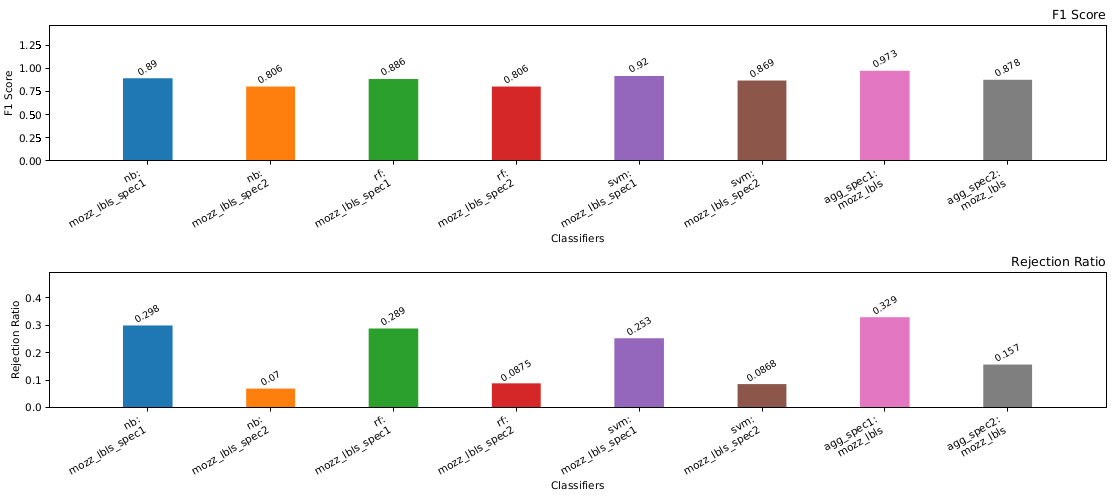
\includegraphics[width=0.8\textwidth]{f1andrej}
            \label{fig:exp-summary-f1andrej}
        }
        \qquad
        \subfloat[][ROC Curves.]{
            \centering
            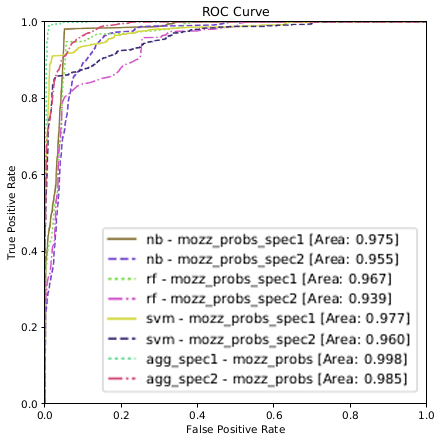
\includegraphics[width=0.3\textwidth]{roc}
            \label{fig:exp-summary-roc}
        }
        \subfloat[][Precision-recall curves.]{
            \centering
            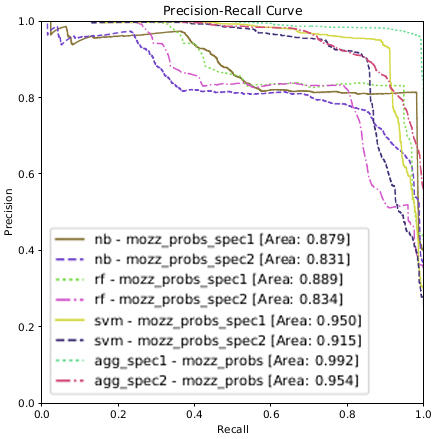
\includegraphics[width=0.3\textwidth]{precrec}
            \label{fig:exp-summary-precrec}
        }
        \caption{Metrics for the best performing models.}
        \label{fig:exp-summary-metrics}
        
    \end{figure}
    Performance measures are shown in figure \ref{fig:exp-summary-metrics}, where results for the best performing individual classifiers are included as well as the aggregated results, for each design specification criteria. Further numerical results are presented in the final rows of appendices \ref{sec:appdx-postproc} and \ref{sec:appdx-agg}.
    
    
    
    